\section{Caracteristicas da melodia}
\label{sec:caracteristicas:melodia}
\index{Musicalidade!Melodia}


Se descrevemos uma \hyperref[sec:pos:Melodia]{\textbf{melodia}} em função das relações existentes entre os tons,
podemos definir as seguintes caraterísticas: 
A extensão (``range'' em inglês),
o contorno  (``shape'' ou ``contour'' em inglês) e 
o movimento  (``movement'' em inglês) 
\cite[pp. 43]{holland2013music} \cite[pp. 50]{langer2017theory}.

\begin{description}
%%%%    %%%%    %%%%    %%%%    %%%%
\item[A extensão melódica:] 
\label{ref:melodica:range}
\index{Musicalidade!Extensão melódica}
Refere-se à extensão entre a nota de maior 
e a de menor \hyperref[sec:pos:Altura]{\textbf{altura}},
 numa melodia ou uma parte dela \cite[pp. 43]{holland2013music}.

\begin{example}[Extensão de uma melodia]
Na pauta descrita na Figura \ref{fig:melody:range:1}, 
vemos uma melodia com uma extensão de 11 semitons, pois a nota mais grave é um dó,
e a mais aguda um si.

Por outro lado se só analisamos uma porção dela, como os 2 primeiros compassos,
então a extensão seria de 7 semitons, pois a nota mais grave é um dó e a mais aguda um sol.
\end{example}
\begin{figure}[!h]
\centering
\href{https://drive.google.com/file/d/1t-idPWPqz53dfPF7Fwtju9xmcIW7ucFw/view?usp=sharing}{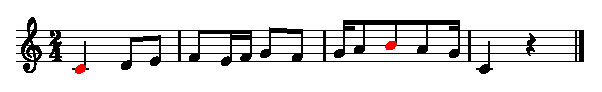
\includegraphics[width=0.99\textwidth]{chapters/cap-musicalidade-percepcion/melodia-carateristicas-range.eps}}
\caption{Rango da melodia.}
\label{fig:melody:range:1}
\end{figure}

Subjetivamente falando, geralmente, as extensões provocam em nós as seguintes reações:
\begin{itemize}
\item Melodias com uma extensão pequena, nos produzem geralmente um clima de calma ou quietude
 \cite[pp. 43]{holland2013music}.
\item Melodias com extensões maiores, nos produzem geralmente uma sensação de liberdade e expansividade
 \cite[pp. 43]{holland2013music}.
\end{itemize}

%%%%    %%%%    %%%%    %%%%    %%%%
\item[O contorno melódico:] 
\label{ref:melodica:shape}
\index{Musicalidade!Contorno melódico}
Refere-se ao contorno criado pelas mudanças de altura de uma melodia;
podemos imaginar o contorno como uma linha formada pelas cabeças das notas musicais 
\cite[pp. 44]{holland2013music} \cite[pp. 61]{chazin2016teaching} \cite[pp. 50]{langer2017theory},
como quando unimos pontos para formar um desenho num livro infantil.


\begin{example}[Contorno de uma melodia]
Se usamos a melodia descrita na Figura \ref{fig:melody:range:1}, então  
o contorno da melodia é descrito pela linha que une as cabeças das figuras musicais,
como mostra a Figura \ref{fig:melody:shape:1}.
\end{example}
\begin{figure}[!h]
\centering
\href{https://drive.google.com/file/d/1t-idPWPqz53dfPF7Fwtju9xmcIW7ucFw/view?usp=sharing}{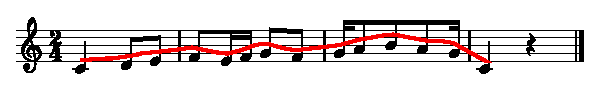
\includegraphics[width=0.99\textwidth]{chapters/cap-musicalidade-percepcion/melodia-carateristicas-shape.eps}}
\caption{Contorno da melodia.}
\label{fig:melody:shape:1}
\end{figure}

Para um dançarino é importante reconhecer o contorno de uma melodia, 
pois assim este pode discernir o \hyperref[ref:climax]{\textbf{clímax}} de cada frase musical, 
e perceber como estas se relacionam com as outras frases musicais
\cite[pp. 45]{holland2013music}.

%%%%    %%%%    %%%%    %%%%    %%%%
\item[O movimento melódico:]
\label{ref:melodica:movimento}
O termo movimento se refere à distancia relativa entre as notas consecutivas de uma melodia;
onde os movimentos melódicos podem ser categorizados como conjuntos ou disjuntos 
\cite[pp. 52]{langer2017theory} \cite[pp. 165]{reinato2010musicavol1} \cite[pp. 45]{holland2013music}. 
\begin{itemize}
\item Um \textbf{movimento melódico conjunto} indica 
\label{ref:melodica:movimento:conjunto}
que as figuras musicais consecutivas
tem sempre \hyperref[sec:intervalomelodico]{\textbf{intervalos}} consecutivos,
ascendentes ou descendentes; estes podem ser intervalos de 
\hyperref[tab:intervalomelodico2]{\textbf{segunda menor}},
\hyperref[tab:intervalomelodico2]{\textbf{segunda maior}} e
os cromáticos  \cite[pp. 165]{reinato2010musicavol1} \cite[pp. 52]{langer2017theory}.  
\item Um \textbf{movimento melódico disjunto} indica 
\label{ref:melodica:movimento:disjunto}
que as figuras musicais consecutivas
se movimentam em \hyperref[sec:intervalomelodico]{\textbf{intervalos}} 
de \hyperref[tab:intervalomelodico2]{\textbf{terça menor}} ou superiores 
\cite[pp. 166]{reinato2010musicavol1} \cite[pp. 53]{langer2017theory}.
\end{itemize}~

\begin{example}[Movimento de uma melodia]
Se usamos a melodia descrita na Figura \ref{fig:melody:range:1},
observamos que esta é conjunta na maior parte dela,
excepto na transição entre o terceiro e quarto compasso,
onde o movimento é disjunto,
como mostra a Figura \ref{fig:melody:movement:1}.
\end{example}
\begin{figure}[!h]
\centering
\href{https://drive.google.com/file/d/1t-idPWPqz53dfPF7Fwtju9xmcIW7ucFw/view?usp=sharing}{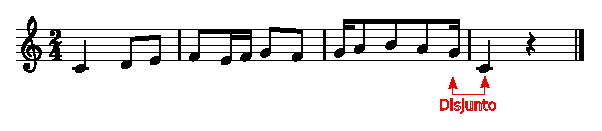
\includegraphics[width=0.99\textwidth]{chapters/cap-musicalidade-percepcion/melodia-carateristicas-movement.eps}}
\caption{Movimento da melodia.}
\label{fig:melody:movement:1}
\end{figure}

As melodias tendem a ser compostas de forma conjunta, 
pois desse jeito são mais fáceis de cantar,
e dependendo do instrumento musical, mais fáceis de executar  
\cite[pp. 53]{langer2017theory}. 

\end{description}~


\PRLsep{Treinamentos}


\begin{example}[Treinamento para reconhecer o contorno melódico:]
Um bom treinamento de percepção melódica,
para que nossa mente esteja preparada para perceber o contorno melódico,
seria escutar de forma aleatória\footnote{Para conseguir a escolha aleatória,
você pode colocar as musicas numa playlist que execute as músicas 
seguindo algum algoritmo pseudoaleatório;
ou também pode pedir a algum amigo que selecione as melodias enquanto você tenta reconhecê-la,
esta forma tem a vantagem que se você não consegue reconhecer na primeira tentativa,
pode pedir a ele repetir a melodia.} 
as melodias que produzem as pautas da Figura \ref{fig:9melodias},
e tentar reconhecer a qual pauta pertencem só pela nossa audição.
\end{example}


\begin{example}[Treinamento para reconhecer a extensão melódica:]
Usando as  pautas mostradas na Figura \ref{fig:9melodias},
poderíamos treinar nossa percepção da extensão melódica,
e tentar reconhecer, escolhendo aleatoriamente as melodias, 
se estas tem uma extensão pequena ou grande.

Além desse treinamento, podemos tentar deduzir qual é a nota musical de menor tom, 
e qual é a de maior tom.
\end{example}


\begin{figure}[!h]
     \centering
     %%%
     \begin{subfigure}[b]{0.3\textwidth}
         \centering
         \href{https://drive.google.com/file/d/1U5BxdQXU9ICCFCV3OnFzpLpB9DjtDFaQ/view?usp=sharing}{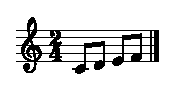
\includegraphics[width=\textwidth]{chapters/cap-musicalidade-percepcion/melodia-chars-shape-1-1.eps}}
         \caption{Melodia 1.}
         \label{fig:melodia-chars-shape-1-1}
     \end{subfigure}
     \hfill
     %%%
     \begin{subfigure}[b]{0.3\textwidth}
         \centering
         \href{https://drive.google.com/file/d/1wp8U3x5Z5lsfeWvAnSuY0UAiRfCeLfce/view?usp=sharing}{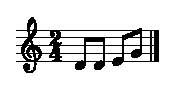
\includegraphics[width=\textwidth]{chapters/cap-musicalidade-percepcion/melodia-chars-shape-2-1.eps}}
         \caption{Melodia 2.}
         \label{fig:melodia-chars-shape-2-1}
     \end{subfigure}
     \hfill
     %%%
     \begin{subfigure}[b]{0.3\textwidth}
         \centering
         \href{https://drive.google.com/file/d/11OGtv8owTiuFJzwmDIudR2kHO5KpfGLY/view?usp=sharing}{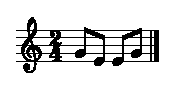
\includegraphics[width=\textwidth]{chapters/cap-musicalidade-percepcion/melodia-chars-shape-3-1.eps}}
         \caption{Melodia 3.}
         \label{fig:melodia-chars-shape-3-1}
     \end{subfigure}
     \hfill
     %%%
     \begin{subfigure}[b]{0.3\textwidth}
         \centering
         \href{https://drive.google.com/file/d/1Yx5ivMcNrHLLv0CE6k1_WaWYHkeFtr0-/view?usp=sharing}{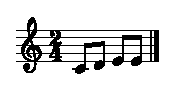
\includegraphics[width=\textwidth]{chapters/cap-musicalidade-percepcion/melodia-chars-shape-4-1.eps}}
         \caption{Melodia 4.}
         \label{fig:melodia-chars-shape-4-1}
     \end{subfigure}
     \hfill
     %%%
     \begin{subfigure}[b]{0.3\textwidth}
         \centering
         \href{https://drive.google.com/file/d/1_61GHFPCOyzDegUuudMwcEmkjrvS0kAG/view?usp=sharing}{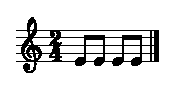
\includegraphics[width=\textwidth]{chapters/cap-musicalidade-percepcion/melodia-chars-shape-5-1.eps}}
         \caption{Melodia 5.}
         \label{fig:melodia-chars-shape-5-1}
     \end{subfigure}
     \hfill
     %%%
     \begin{subfigure}[b]{0.3\textwidth}
         \centering
         \href{https://drive.google.com/file/d/1YRUrgJvnkGlmMI7UV1UwOmRJH3VBrzcq/view?usp=sharing}{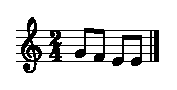
\includegraphics[width=\textwidth]{chapters/cap-musicalidade-percepcion/melodia-chars-shape-6-1.eps}}
         \caption{Melodia 6.}
         \label{fig:melodia-chars-shape-6-1}
     \end{subfigure}
     \hfill
     %%%
     \begin{subfigure}[b]{0.3\textwidth}
         \centering
         \href{https://drive.google.com/file/d/1jRZEfsaEXEPIDIarktZA7FK0dQ8xE4B0/view?usp=sharing}{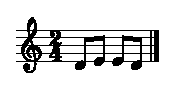
\includegraphics[width=\textwidth]{chapters/cap-musicalidade-percepcion/melodia-chars-shape-7-1.eps}}
         \caption{Melodia 7.}
         \label{fig:melodia-chars-shape-7-1}
     \end{subfigure}
     \hfill
     %%%
     \begin{subfigure}[b]{0.3\textwidth}
         \centering
         \href{https://drive.google.com/file/d/11SZQvNkkYqM6qyZblaxMEV1fB0ysIlxH/view?usp=sharing}{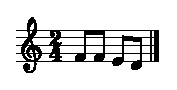
\includegraphics[width=\textwidth]{chapters/cap-musicalidade-percepcion/melodia-chars-shape-8-1.eps}}
         \caption{Melodia 8.}
         \label{fig:melodia-chars-shape-8-1}
     \end{subfigure}
     \hfill
     %%%
     \begin{subfigure}[b]{0.3\textwidth}
         \centering
         \href{https://drive.google.com/file/d/1gX_eJdsTBCEY2PBFP7ZS6HIeqgw-p-Ut/view?usp=sharing}{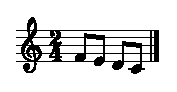
\includegraphics[width=\textwidth]{chapters/cap-musicalidade-percepcion/melodia-chars-shape-9-1.eps}}
         \caption{Melodia 9.}
         \label{fig:melodia-chars-shape-9-1}
     \end{subfigure}
     \hfill
        \caption{Tipos de contornos melódicos}
        \label{fig:9melodias}
\end{figure}



